%This template is based on one provided by the American Physical Society for submission to its journals.

\documentclass[aps,twocolumn,showpacs,preprintnumbers]{revtex4}

%The following packages add LaTeX commands that make formatting and writing math easier

\usepackage{graphicx}  % Include figure files
\usepackage{subfigure}
\usepackage{multirow}
\usepackage{verbatim}

\linespread{1.1}
\usepackage{fancyhdr}
\usepackage{longtable}
\usepackage{parskip}
\usepackage[T1]{fontenc}
\usepackage{dcolumn}   % Align table columns on decimal point

\usepackage{bm}        % bold math
\usepackage{amsfonts}  % Common math fonts
\usepackage{amsmath}   % Common math functions
\usepackage{amssymb}   % Common math symbols
\usepackage{physics}

%The following custom commands simplify commonly used LaTeX commands

\newcommand{\pic}[2]{\begin{center} \includegraphics[scale=#1]{#2}\end{center}}
\newcommand{\re}[1]{\mathrm{Re}\left(#1\right)}
\newcommand{\im}[1]{\mathrm{Im}\left(#1\right)}
\newcommand{\bdot}[1]{\dot{ \bb {#1}}}
\newcommand{\bddot}[1]{\ddot{ \bb {#1}}}
\newcommand{\bidot}[1]{\dot{ \bi{ #1}}}
\newcommand{\biddot}[1]{\ddot{ \bi {#1}}}
\newcommand{\ep}{\varepsilon}
\newcommand{\for}{\quad \quad \mathrm{for} \quad\quad}
\newcommand{\then}{\quad \quad \implies \quad\quad}
\newcommand{\an}{\quad \quad \mathrm{and} \quad\quad}
\newcommand{\ifff}{\quad \quad \mathrm{if} \quad\quad}
\newcommand{\where}{\quad \quad \mathrm{where} \quad\quad}
\newcommand{\dg}{^\dagger}
\newcommand{\semi}{\quad \quad \mathrm{;} \quad\quad}
\newcommand{\paren}[1]{\left( #1 \right)}
\newcommand{\brac}[1]{\left[ #1 \right]}
\newcommand{\bra}[1]{\left\langle #1 \right|}
\newcommand{\exv}[1]{\left\langle #1 \right\rangle}
\newcommand{\pwisein}{\left\{ \begin{array}{ll}}
\newcommand{\pwiseout}{\end{array}\right.}
\newcommand{\ket}[1]{\left| #1 \right\rangle}
\newcommand{\bracket}[2]{\left\langle #1 | #2 \right\rangle}
\newcommand{\trace}[1]{\mathrm{Tr} \left( #1 \right)}
\renewcommand{\det}[1]{\mathrm{det}\left( #1 \right)}
\newcommand{\del}[1]{\frac{\partial}{\partial #1}}
\newcommand{\fulld}[1]{\frac{d}{d #1}}
\newcommand{\fulldd}[2]{\frac{d #1}{d #2}}
\newcommand{\dell}[2]{\frac{\partial #1}{\partial #2}}
\newcommand{\delltwo}[2]{\frac{\partial^2 #1}{\partial #2 ^2}}
\newcommand{\bb}{\mathbf}
\newcommand{\bi}{\boldsymbol}
\newcommand{\eq}[1]{\begin{equation} #1 \end{equation}}
\newcommand{\radhalf}{ \frac{ \sqrt{2}}{2}}
\newcommand{\sigx}{\left( \begin{array}{cc} 0 & 1\\ 1 & 0 \end{array}\right)}
\newcommand{\sigy}{\left( \begin{array}{cc} 0 & -i\\ i & 0 \end{array}\right)}
\newcommand{\sigz}{\left( \begin{array}{cc} 1 & 0\\ 0 & -1 \end{array}\right)}
\renewcommand{\matrix}[1]{\left( \begin{array} #1 \end{array}\right)}
\newcommand{\thermo}[3]{\left( \frac{\partial #1}{\partial #2} \right)_{#3}}
\newcommand{\coolfrac}[2]{\left( \frac{ #1}{ #2} \right)}

\setlength{\parindent}{10pt}

\begin{document}

\title{Gravity Tunnel through the Earth using  an effective mass density function}

\author{Nicolás Gómez, Carlos Quimbay}

\affiliation {\it Departamento de Física, Universidad Nacional de Colombia, Bogotá D.C., Colombia}

\date{\today}

\begin{abstract}  

%FIRST ATTEMPT
%The gravity tunnel problem is faced with the use of a decreasing power law function as the mass density. Some parameters are introduced and determined to find a concordance between the traversal times found using the density profile from seismic data and the power law function. A trustworthy concordance is found in traversal times, velocity profiles and shapes of the braquistochrones , making our proposition an effective mass density function that can describe the interior of the Earth.

%SECOND ATTEMPT

A novel effective function for the mass density profile inside the Earth is proposed in order to describe qualitatively and quantitatively physical aspects of the terrestrial density derived from seismic models. This was done using a decreasing potential law function dependent only on the distance to the center of the Earth and on some parameters, in such a way that central density, surface density and total mass are correctly given. This effective function was applied to gravity tunnel concepts as a test of the predictive power of the effective model, but the comparison is established with the geophysical approach predictions, in the place of real life experiments, due to the impossibility of performing this. A high correspondence between the effective model and the reference model was found. 

\end{abstract}


\maketitle 

\section{Introduction}

    A gravity tunnel is a hypothetical means of transportation in which, to arrive to one point to another on the surface of the planet, it appeals to the acceleration of gravity in a tunnel connecting both points. The problem is clearly pedagogic and has been thoroughly discussed in journals of this character. \citep{History-Tunels}. 
    
    This has been made in a lot of different ways, considering the simplest case of constant density\citep{Venezian}, proposed as exercise in classical mechanics  textbooks\cite{Goldstein}, adding rail's friction \citep{Tunel-friccioon}, or considering the rotation of the Earth \citep{Solomon2, Iserman2, Simonic}, and the effect of this in its geometrical form\citep{Taillet2018}, or even in the frame of general relativity \citep{Parker2017, Seel}. Likewise, this has been done considering density-pressure relations based on polytropes \citep{Tunel-Potencia, Politropes2}, or in more accurate density geophysical models as the Preliminary Reference Earth Model (PREM), being this last one done numerically by Klotz \citep{gravity-train-prem},
    making a comparison with a constant gravity approximation; and also doing an analytical treatment using a linear, piecewise approximation which throw closer results to those of the PREM, and which get out the poorly physical situation of a constant gravity  (since this implies infinitive densities at the center of the planet).\citep{gravity-train-prem-approx, Iserman2}. 

    For geophysical, astrophysical, as well as purely physical purposes, knowing the density distribution inside of our planet is of great utility. In a first approximation and to uniquely illustrative aims, it can be taken to be constant, dividing total mass under its volume and getting $\Bar{\rho}=5513kg/m^3$ \citep{AstronomicalConstants}.
    
    With this one can obtain approximate values for the acceleration of gravity or moments of inertia. Nevertheless, it is clear that the density on Earth (and on any astronomical body) is far from being constant. Other models have been proposed in order to describe the density \citep{Snyder1985} or the acceleration \citep{Dragoni2020} of our planet, but the most accepted model is the Preliminary Reference Earth Model, according to which the density in the interior has discontinuities between the different layers that form it: inner core, outer core, mantle and crust. Inside each region, density can be approximated with a polynomial function\citep{PREM} . This can be seen on figure \ref{fig:Prem density}. Notice that density increases towards the center and reaches its maximum value around $ 13000kg/m^3$, while in the surface is $1020kg/m^3$, which corresponds to the density of the water in the ocean.
    
    In the present work it is intended to discuss a possible approximation to this model using an effective density function more simple to express: soft, continuous and certainly not constant.  This function is contemplated as a possible replacement to the described for the Reference Model and, thus, as a simple but accurate description of Earth physical effects.
    
    \begin{comment}
    Two profiles are used, given by decreasing power law functions, using two and three parameters, among them, the power itself, to get from it the most physics possible. What we meant is that our effective density function accounts for the gravitational acceleration on the surface, $g=9.81 m/s^2$ and for the traversal times in a gravity tunnel, with respect to those obtained in \citep{gravity-train-prem} for the PREM description. 
    \end{comment}
    
    The use of this function not only represents a totally different treatment compared to those previously mentioned for the treatment of the gravity tunnel, but also serves as an example to illustrate the construction and the development of an effective model. Effective models in classical mechanics and, actually in undergraduate physics, are very rare. Nonetheless its utility  in the scientific world is becoming greater and greater; hence, it is important that students at this level in a physics or engineering career get familiar with some model with a simple and fairly known physics and that doesn't contain any complicated mathematical or computational methods. The present article accomplish all those requirements due to the simple deductions, presented in the field of Newton mechanics, and to the functions used, which are integrable  either in analytical form or with the conventional numerical methods.

    For the effective density function construction, the density profiles are first raised in section \ref{density section}, were conditions over the parameters to fix are stated. Total mass and gravity are computed as consistency checks in section \ref{consistency checks section}, then, speed profiles, traversal times and brachistochrone shapes are computed and compared in \ref{Predictions section}. 
    
    Finally, in \ref{acceleration section}, we study the acceleration along the path, in order to give a dynamic explanation of why the times are shorter for longer paths such as brachistochrone, and not for the paths of shorter distance.

    \begin{figure}
        \centering
        \includegraphics[scale=0.6]{Figures/prem-profile.pdf}
        \caption{Density on the inside of the Earth as a function of the radius according to the data obtained by PREM.}
        \label{fig:Prem density}
    \end{figure}




    
\section{Density Profile}\label{density section}

    In order to account for a density that replaces the one in fig. \ref{fig:Prem density}, with a continuous and soft form, but such that it reproduces the following geophysical situations 
    
    \begin{enumerate}
        \item Density in the center of the Earth is the same of PREM:
        
        \begin{equation}
            \rho(r = 0) = \rho_c = 13088.5 kg/m^3,
            \label{1 - Density condition in the center}
        \end{equation}
        
        \item Density in the surface is that of sea water
        
        \begin{equation}
            \rho(r=R) = \rho_s = 1020kg/m^3,
            \label{1 - Density condition in the surface}
        \end{equation}
        
        \item Total mass is the reported mass of the Earth
        
        \begin{equation}
        \begin{aligned}
            \mathcal{M}(r=R) = 4 \pi \int_0^{R} \rho(r) r^2 dr \\
                      M_T = 5.97 \times 10^{24} kg; 
        \end{aligned}   
        \label{1 - Density condition, total mass}
        \end{equation}
    \end{enumerate}
    and such that it allows to make predictions, we have considered the following decreasing power law binomial function of three parameters:
    
    \begin{equation}
        \rho(r; b, c, d) = \Bar{\rho} b \left( 1 - c \frac{r}{R}\right)^d,
        \label{1 - General density form}
    \end{equation}
    with $\Bar{\rho} = 3M_T/4 \pi R^3 = 5513\; kg/m^3$ the average density on the Earth, and $b, c, d$ all real and positive (and $c < 1$). 
    
    The aim of this section is to apply conditions \eqref{1 - Density condition in the center} - \eqref{1 - Density condition, total mass} to \eqref{1 - General density form} in order to find the parameters $b,c,d$ that constitute our effective model of the density.
    
    \subsubsection{First Condition: Central density}
    
    With the given function, in the center $r = 0$, we have
    
    \begin{equation}
    \begin{aligned}
        \rho(0) =& \Bar{\rho} b = \rho_c \\ 
                \rightarrow & b = \rho_c / \Bar{\rho} = 2.372,
    \end{aligned} 
    \label{1 - First condition, equation}
    \end{equation}
    the firs of the parameters, $b$, was easily fixed. The reader shouldn't expect the same for the other two. 
    
    \subsubsection{Second Condition: Surface density}
    
    In the surface ($r=R$), the expression seems simple, but still depends on the remaining parameters:
    
    \begin{equation}
    \begin{aligned}
        \rho (R ) =& \Bar{\rho} b (1 - c)^d = \rho_s \\
        \rightarrow& (1-c)^d = \frac{\rho_s}{\Bar{\rho} b} = 0.0764.
    \end{aligned}
     \label{1 - Second condition, equation}
    \end{equation}
    In principle, one could solve one in terms of the other but this doesn't help for an analytical solution of the system of equations.
    
    \subsubsection{Third Condition: Total mass}
    
    For this last condition, for a general $c$ and $d$ we have:
    
    \begin{align*}
        M_T  =& 4 \pi \Bar{\rho} b \int_0^R \qty(1 - c \frac{r}{R} )^d r^2 dr \\
        =&  \frac{4 \pi \Bar{\rho} b[2 - (1-c)^{d+1} (2 + 2c (1+d) + c^2 (2 + 3d + d^2))]}{c^3 (6 + 11d + 6 d^2 + d^3)}.
    \end{align*}
    Naturally, the best way to perform such an integration is with the aid of a symbolic programming software, in our case we used \textit{Mathematica}.
    
    Back to the equation, noticing that $\Bar{\rho}$ can be written in terms of $M_T$ in such a way that they cancel, we end up with the following equation for the third condition:
    
    \begin{equation}
         \frac{ 3 b[2 - (1-c)^{d+1} (2 + 2c (1+d) + c^2 (2 + 3d + d^2))]}{c^3 (6 + 11d + 6 d^2 + d^3)} = 1.
         \label{1 - Third condition, equation}
    \end{equation}
    With the system of two equations \eqref{1 - Second condition, equation} and \eqref{1 - Third condition, equation} we can solve for the two variables $c, d$ using the definition of $b$, \eqref{1 - First condition, equation}. A proper code gives the following results for this equations:
    
    \begin{align*}
        b &= 2.373, \\
        c &= 0.9875, \\
        d &= 0.5867.
    \end{align*}
    
    With this values we define our effective density function $\rho (r)$, which is plotted in Fig. \eqref{fig: 1- density} with the PREM profile for comparison.
    
    \begin{figure}
        \centering
        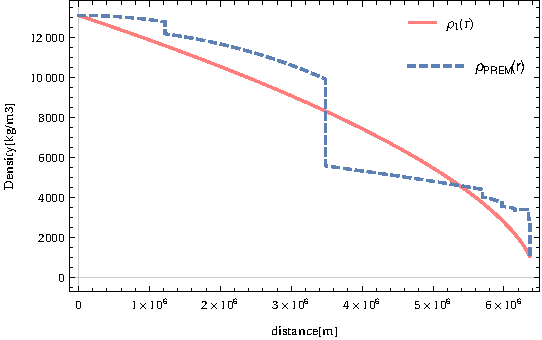
\includegraphics[scale=0.85]{Figures/1-densities.pdf}
        \caption{Effective density function plotted along with numeric profile of PREM (dashed lines).}
        \label{fig: 1- density}
    \end{figure}
    
\section{Numerical consistency tests for the effective model} \label{consistency checks section}
    
In this section, we want to use the effective density function found to check if the numerical computation of some quantities is correct, giving us a first clue of the correctness of the method elaborated. 
    
    \subsubsection{Total mass}
    
    The test of the first two conditions is trivial and it's just the minimum requirement. With all the digits we have checked that the condition values are returned. Let's consider now the integration of the density to find the mass, which is less immediate. With any integration algorithm, it can be seen that the following integral
    
    \begin{equation*}
         4\pi \times 2.374 \Bar{\rho} \int_0^R (1 - 0.9869 r/R)^{0.5881} dr ,
    \end{equation*}
    gives,
    
    \begin{equation*}
        M_T = 5.972 \times 10^{24} \; kg
    \end{equation*}
    the value reported in the literature. So far so good.
    
    \subsubsection{Acceleration of gravity}
    
    The acceleration of gravity in the surface is another physical constant that must be appropriately given by our effective model. This is, however, not a prediction. Thanks to Newton's shell theorem, total mass is what gives gravity its constant value on the surface, regardless of the distribution of mass. This fact can also be seen in the mathematical expression derivable from Gauss law (the integrals are the same):
    
    \begin{equation}
        a (r) &= \frac{4 \pi G}{r^2}  \int_0^r \rho (r') {r'}^2 dr'.
        \label{1 - acceleration from Gauss law}
    \end{equation}
    
    The interest we have in the form of the acceleration, not only in the surface but in the inside as well, is that, to perform the predictions of the model within the context of the gravity tunnel, we will need this as a function of the radius. Furthermore, there are two ways to address this and some of the next computations. One is integrating by brute force eq. \eqref{1 - acceleration from Gauss law}, as we did with the expression of $M_T$. The other is re-writing the density using Newton's binomial theorem 
    
     \begin{equation*}
        \rho(r; b,c,d) = \Bar{\rho} b \sum_{k= 0}^{\infty} \binom{d}{n} (-c)^k \qty( \frac{r}{R} )^k.
    \end{equation*}
    Both methods lead to analytical expressions for accelerations and velocities (although very cumbersome for the former one), but next computations as traversal times and brachistochrone shapes must be done numerically. The effectiveness with which these can be done could depend on one method or the other, as well as the programming algorithms. We will only show the results here and develop the equivalence on the appendix, for the interested reader to see an application of the generalized binomial theorem.
    
    In this way, the gravity on the surface with any of the approaches gave us
    
    \begin{equation*}
        g = 9.816 \; m/s^2,
    \end{equation*}
    which is the average gravity at see level. In the whole range, compare with PREM data, is as depicted on Fig. \ref{fig: 1- gravity}.
    
    \begin{figure}
        \centering
        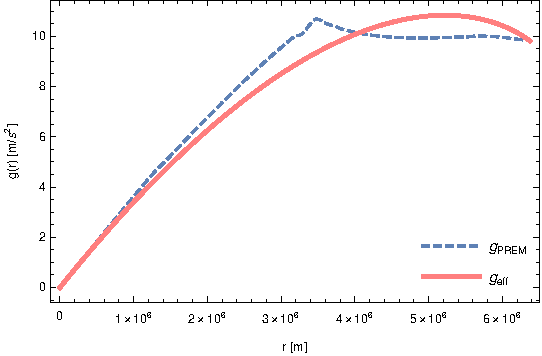
\includegraphics[scale=0.85]{Figures/3-accelerations.pdf}
        \caption{Acceleration profiles according to PREM data and to effective density function.} 
        \label{fig: 1- gravity}
    \end{figure}
    
    One can notice that the whole distribution is not so close at all points, but this hardly could have been the case, given the functional form of PREM profile. Still, we think the effective gravity found is close enough and nicely smooth; so the least requirements for the model are fulfilled. 
    
\section{Predictions for the gravity tunnel problem}   \label{Predictions section}

With the confidence on our effective density function gained above, and with the help of some physical quantities already covered, we can test the prediction power of the model. Keep in mind that, in contrast with effective model in real world, our predictions can not be tested experimentally, so we rely on the same quantities computed directly from PREM. In the next subsections we use both and compare the results.
    
    \subsection{Velocity profile}\label{velocity section}
    
    Once the mass distribution within the physical sphere to be considered is known, the speed followed by a test particle while inside it can be found from energy considerations. In the first instance, at any point we have
    
    \begin{equation*}
        E = \frac{1}{2} m v^2(r) + U(r),
    \end{equation*}
    and, given that $E$ is a constant of the motion, a change in potential energy
    
    \begin{equation*}
        \Delta U = G m \int_{r_1}^{r_2} \frac{M(r')}{{r'}^2} dr'  ,
    \end{equation*}
    is accompanied by a change in the velocity. The simplest case to consider is $r_1 = R$, and supposing a zero velocity, we obtain in terms of the density 
    
    \begin{equation}
        \frac{v^2(r)}{2} = 4 \pi G \int_{r}^{R} \frac{1}{{r'}^2} \int_{0}^{r'} \rho(r'') {r''}^2 dr'' dr' .
        \label{1 - v profile, general form}
    \end{equation}

    Using now \eqref{1 - General density form} with the above given values in the velocity profiles, an incredible coincidence can be observed (see Fig. \ref{fig: 1- velocity}). 
    
    \begin{figure}
        \centering
        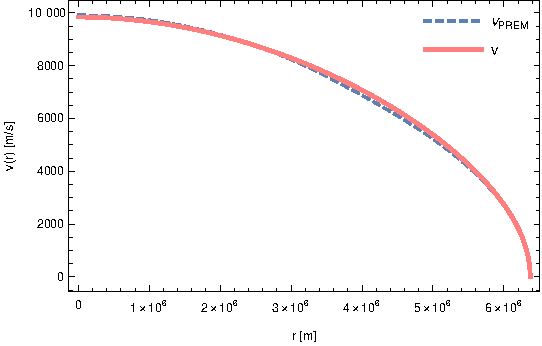
\includegraphics[scale=0.85]{Figures/4-velocities.pdf}
        \caption{Velocity profile of the model along with the one obtained from the effective density, for the path between antipodes.}
        \label{fig: 1-velocity}
    \end{figure}
        
    The maximum velocities in the antipodean trajectories predicted by each function are decently close
    
    \begin{align*}
        v_{PREM}(0) &= 9915 \; m/s, \\
        v_{eff} (0) &= 9840 \; m/s 
    \end{align*}
    this means an error for the velocities of

    \begin{equation*}
        \Delta v = 0.8 \%
    \end{equation*}
    
    
    
    \subsection{Traversal time}\label{time section}
        
    Taking $ ds ^ 2 = dr ^ 2 + r ^ 2 d \theta ^ 2 $ as the infinitesimal interval of a trajectory, and $ v (r) $ the instantaneous velocity of an object on this trajectory as a function of $ r $. The travel time is given by
   
            
    \begin{equation*}
        t = \int \frac{ds}{v(r)},
    \end{equation*}
    that can be more conveniently rewritten as
            
    \begin{equation}
        t = \int \frac{\sqrt{r^2 + {r'}^2}}{v(r)} d\theta = \int \frac{\sqrt{ 1 + r^2 {\theta'}^2}}{v(r)} dr, 
        \label{1 - times}
    \end{equation}
    with $ {r '} = dr / d \theta $ and $ \theta' = d \theta / dr $. Either of the two possibilities of \eqref{1 - times} can be used as convenient, depending on the description needed for the trajectory to be considered. In our case, as in most of the literature, we are going to consider chord trajectories (minima of distance) and brachistrochrone trajectories (minima of time). But let's begin with the simplest of all the cases: the path joining diametrically opposite points, or antipodes.

        \subsubsection{Traversal time between antipodes}
    
        This path is the first to be considered in all the literature on the subject because it is clearly the simplest case, and in the case of constant density it gives a traversal time $ T_0 = 42 \text{min } $ \citep{History-Tunels}. In the assumption of constant gravity we obtain $ T_{\text{const}} = 37 \text{min } 58 \text{s} $, the numerical expression of PREM gives $ T_{\text {prem}} = 38 \text{min } 11 \text{s } $ \cite{gravity-train-prem}, while in our case, using the right part of \eqref{1 - times} with $ \theta'= 0 $ and the speed profile \eqref{1 - v profile, general form} gives
        
        \begin{align*}
            T_{eff} &= 37 \text{min}  \hspace{0.1cm} 45 \text{s}
        \end{align*}
        which represents a discrepancy with respect to the model of
        
        \begin{equation*}
            \Delta T = 1.1 \% .
        \end{equation*}
        Remember we are comparing our results not with real world data, but with other model. If someone were to do the ``experiment'', the time taken to travel the Earth surely would no be exactly $T_{PREM}$, and we expect that at least our prediction $T_{eff}$ would be within the uncertainty of that experiment, but we will never know it.
        
        We now proceed to calculate the times in other trajectories.
                
        \subsubsection{Chord Path}
    
        In terms of the parameter $ d $ ( the shortest distance between this line to the center of the sphere (see Fig. \ref{fig: 1- Earth drawing})), the trajectory can be written as the relation
            
        \begin{figure}
            \centering
            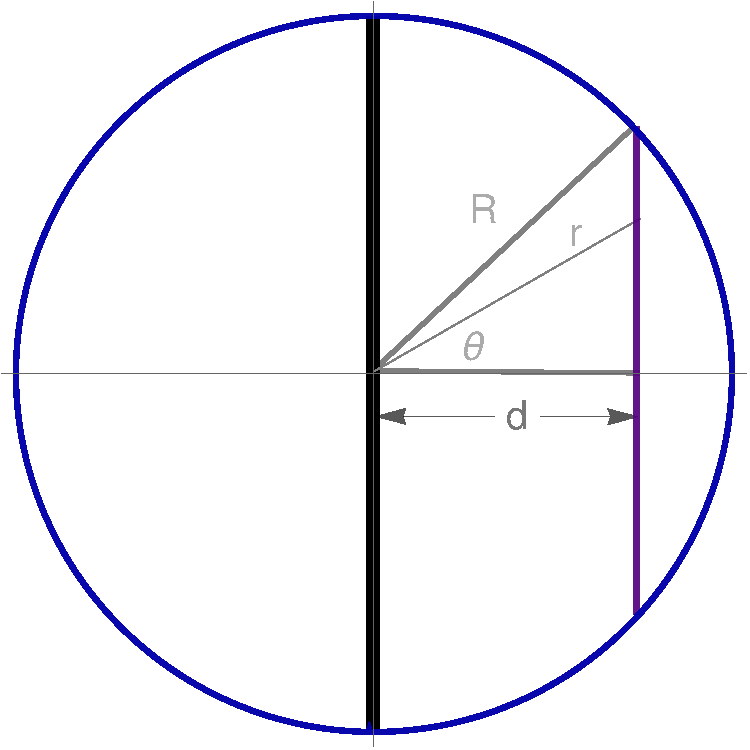
\includegraphics[scale=0.55]{Figures/earthdrawing.pdf}
            \caption{Representation of the Earth and the chord path at a distance $d$, with other useful parameters.}
            \label{fig: 1- Earth drawing}
        \end{figure}    
            
        \begin{equation*}
            r = \frac{d}{\cos{\theta}}
        \end{equation*}
                
        with this, the right integral in \eqref{1 - times} becomes
            
        \begin{equation*}
            t = \int \frac{r}{\sqrt{r^2 -d^2}} \frac{dr}{v(r)},
        \end{equation*}
        Now considering the limits, $ r $ takes a maximum value equal to the radius of the sphere $ R $, down to a minimum value $ d $, to return to $ R $ at the other end. The times to solve are found then by
        
        \begin{equation}
            \frac{T}{2} =  \int_{d}^{R} \frac{r}{\sqrt{r^2 -d^2}} \frac{dr}{v(r)}.
            \label{1 - Times for chord path}
        \end{equation}
        
        In Fig. \ref{fig: 1-times}, despite the lack of an incredible coincidence between both functions resulting from the effective density and that from the geophysical model, we see the same particularity that occurs in this type of trajectories, namely, that times, contrary to intuition, are by a few minutes greater the shorter the distance.
            
        \begin{figure}
            \centering
             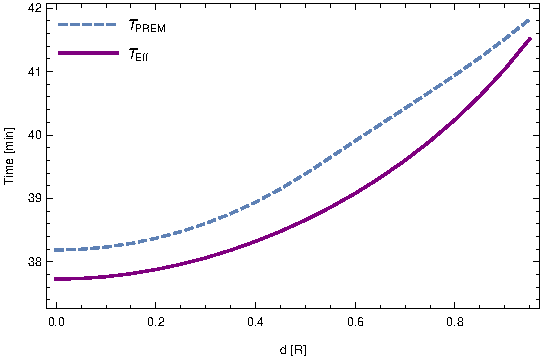
\includegraphics[scale=0.85]{Figures/5-chordtimes.pdf}
            \caption{Traversal time for the chord path between two arbitrary points on the surface as a function of the distance $d$ of the path to the center of the Earth.}
            \label{fig: 1-times}
        \end{figure}
            
            
    \subsection{Brachistochrone Path}\label{braquistochrone section}
        
    The brachistochrone curve is by definition the one in which the descent or route takes the least time, or in the same way, in which the speeds reached are the greatest. To find these curves, as usual, variational methods are used on \eqref{1 - times} and the respective Euler-Lagrange equations are found. To do this, take the integral on the left, so that
    
    \begin{equation*}
        t = \int f(r, r', \theta) d\theta,
    \end{equation*}
    with
            
    \begin{equation}
        f= \frac{\sqrt{r^2 + (dr / d\theta )^2 } }{v(r)}, 
        \label{1 - effective lagrangian}
    \end{equation}
    which is minimum if 
    
    \begin{equation}
       \frac{d}{d \theta } \left( \frac{\partial f}{\partial r'} \right)  - \frac{\partial f}{\partial r} = 0 ,
       \label{1 - Euler-Lagrange eqs}
    \end{equation}
    and from \eqref{1 - Euler-Lagrange eqs} we can find, integrating, the trajectories $ r = r (\theta) $. 
    
    Without knowing the speed explicitly, it is possible to develop this equation using the chain rule, and thanks to the non-dependence on $ \theta $,
    
    \begin{equation*}
        r' \frac{\partial f}{\partial r'} - f = c ,
    \end{equation*}
    explicitly
    
    \begin{equation*}
        \frac{1}{v(r)} \frac{{r'}^2}{\sqrt{{r'}^2 + r^2}} - \frac{\sqrt{{r'}^2 + r^2}}{v(r)} = c.
    \end{equation*}
    
    The constant is held at any time along the path, particularly if $ r \rightarrow r_ {min} = d $, where $ r '= 0 $, so that
    
    \begin{equation*}
        c = -\frac{d}{v(d)},
    \end{equation*}
    whereby
    
    \begin{equation*}
         \frac{1}{v(r)} \frac{{r'}^2}{\sqrt{{r'}^2 + r^2}} - \frac{\sqrt{{r'}^2 + r^2}}{v(r)} =   -\frac{d}{v(d)},
    \end{equation*}
    and, in general, the  Euler-Lagrange eq. is
    
    \begin{equation*}
        \frac{r^2}{\sqrt{{r'}^2 + r^2}} = d \frac{v(r)}{v(d)},
    \end{equation*}
    solving for $r'$
    
    %\begin{equation*}
    %    {r'}^2 + r^2 = \frac{r^4 }{d^2} \left( \frac{v(d)}{v(r)} \right)^2
    %\end{equation*}
    
    %or
    
    \begin{equation}
        r' = \left[ \frac{r^4 }{d^2} \left( \frac{v(d)}{v(r)} \right)^2 - r^2  \right]^{1/2} =  \theta'^{-1}(r),
        \label{1 - theta p inverse as function of r,d} 
    \end{equation}
    lastly, the trajectory can be found using
    
    \begin{equation}
        \theta(r) = \int_{d}^{r} \theta' (x) dx.
        \label{1 - trajectory integral}
    \end{equation}


    \begin{figure}
    \centering
    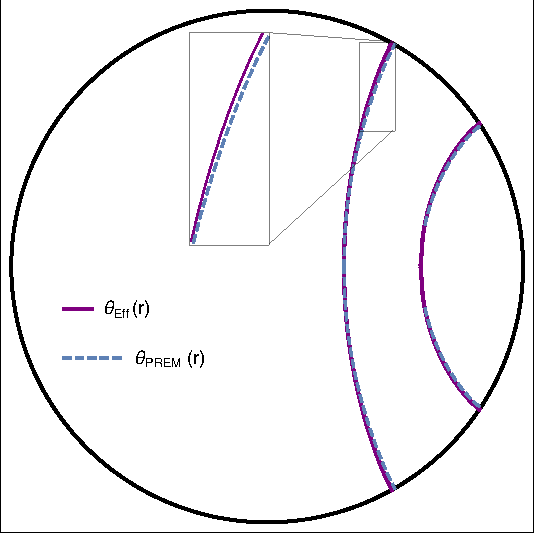
\includegraphics[scale=0.8]{Figures/6-braqShapes.pdf}
    \caption{Shape of the brachistochrone curves for the PREM density and for the effective density }
        \label{fig:1-braquistochrone}
    \end{figure}

        \subsubsection{Times for the brachistochrone path}
        
        The times for this path can be used again with \eqref{1 - times} (in this case $ \theta'$ is the one in \eqref{1 - theta p inverse as function of r,d}), and the same velocity functions. For the two cases that we worked on in this paper, these can be seen in \ref{fig:1-braquistochrone times}. As for the closeness that the functions have to each other, this is a good indication that the physics is the same. So that, for the present treatment, little is lost by replacing the numerical profile of the PREM model with effective densities. Regarding the behavior of two three functions, which is the same for any other density function, the times are lower if the paths connect closer points on the surface, which is to be expected. In addition, the times are, for any given trajectory with an approach $ d $, always smaller than those of straight paths, except for the case $ d = 0 $ in which the trajectories, of course, are the same and therefore so are their traversal times.
        
        \begin{figure}
            \centering
            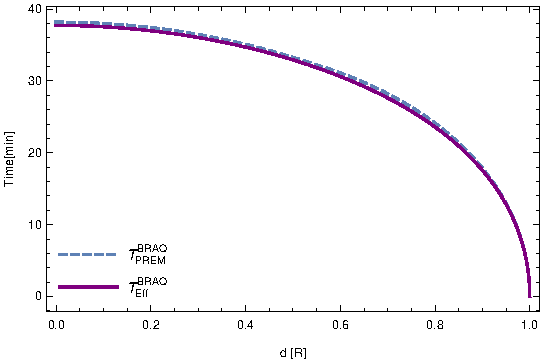
\includegraphics[scale=0.90]{Figures/7-braqTimes.pdf}
            \caption{Traversal time for the brachistochrone paths as a function of the minimum distance of the trajectory to the center of the Earth.}
            \label{fig:1-braquistochrone times}
        \end{figure}
        
        Why the times of the straight paths are greater if the path is shorter, and why a brachistochrone, with respect to a straight path, connecting the same two points on the surface, takes a shorter time to travel, being the length of the tunnel greater, lies in the same justification for all kinematic motion: dynamics. The results obtained for these times, which, as mentioned, are not caused by the density but by the shape of the trajectories itself, when the density depends only on the distance to the center of the Earth, will be justified in the next section.
    
    
        
\section{Acceleration}  \label{acceleration section}
    
    Little has been discussed in the literature on acceleration in the direction of motion for each trajectory. It is true that all the analysis, just as it can start from a given density distribution, can also be done from a gravity profile, and it is in fact as it has been taken in this and other works for the situation of the Earth according to PREM (since these data were also given in the original study \cite{PREM}). However, the vector character of this acceleration also plays a crucial role in understanding which path will take the least time.
    
    In general, the value of the times is understood as the result of a contrast of the length of the paths (decreasing) and the magnitude of the speeds at each point (also decreasing), without fully understanding why one overcomes the other in each case. Studying the accelerations and their components in the direction of the path helps not only to visualize which of these two magnitudes favors the value of the time found but also gives an explanation as to why.  Ultimately, what is done is an analysis of the gravitational attraction on a test body of unit mass, so that
   
    \[ \Vec{F}_g (r) = \Vec{a}_r (r) ,\]
    these accelerations have already been calculated and appear in Fig. \ref{fig: 1- gravity}. Now, these quantities correspond to the value of the acceleration in the radial direction ($ \hat{r} $). To find the magnitude of these accelerations in the direction of the trajectories, we must consider
    
    \[ a(r) = a_r \sin{\theta} ,\]
    for the case of chord paths this corresponds to
    
    \[ a_{CHORD}(r) = a_r(r) \frac{\sqrt{r^2 - d^2}}{r}, \]
    while for the brachistochrone trajectories we use the result found in \eqref{1 - theta p inverse as function of r,d},
    
    \[ a_{BRAQ}(r) = a_r(r) \sin{\left(\theta(r)\right)}. \]
    These results are plotted in the Fig. \ref{fig: 1-a-chord and a-braq} starting only from the acceleration $ a_{PREM} $ in \eqref{1 - acceleration from Gauss law} (at this point the reader is expected to agree that the graphs for $ a_{r eff} $ will be very similar). The six curves correspond to $ a_{CHORD} (r) $ in three straight tunnels connecting different points on the surface (pink color online), and to $ a_{BRAQ} $ for three tunnels that in principle connect the same points on the surface (purple), for this reason they are both on the surface ($ r / R = 1 $). Note also that the closest approach distance $ d $ is smaller in brachistochrone with respect to straight paths, as is also observed in the shape of the trajectories. Also, the value of the acceleration at that point of closest approach is always zero, since the tangent of the path is always perpendicular to the radius.    
        
    \begin{figure}
        \centering
        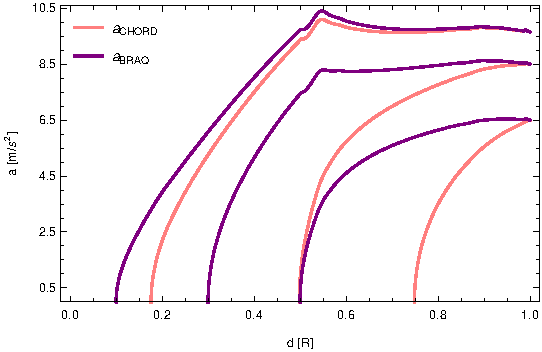
\includegraphics[scale=0.85]{Figures/8-Acceleration-chord-braq.pdf}
        \caption{Acceleration in the direction of the movement for three chord paths (pink online) and for three brachistochrone  paths (purple online).}
        \label{fig: 1-a-chord and a-braq}
    \end{figure}
    
    Regarding the values of the accelerations, which is what concerns us here, two points must be highlighted:
        
    \begin{itemize}
        \item Comparing the accelerations in the straight path, those that correspond to a smaller $ d $, that is, that connect two points farther away on the surface and whose path is longer, are always above those of smaller $ d $, that is, for these paths the acceleration is greater at all points of the trajectory than for shorter paths, and therefore, their speeds are greater, wherewith, the times are shorter.
        \item The same behavior can be observed between the accelerations of the brachistochrones (in magenta) and those of the straight paths (in red). The former are always above, which implies that their speeds are in fact always higher and the times, consequently, lower.
    \end{itemize}
    
    \newline



\section{Conclusion}

    As mentioned, effective models in physics can have great predictive power, despite not being describing the real nature of objects. In the present work we have found, successfully, that the predictions of a function as a law of decreasing power can agree with those obtained using a more descriptive model of the interior of the Earth, when addressing the problem of the gravitational tunnel. Although the shape of the chord times profile is not the best fit to those of the numerical model (see Fig. \ref{fig: 1-times}, there is a great agreement between the velocity profiles (Fig. \ref{fig: 1- velocity}) or brachistochrone shapes (Fig. \ref{fig:1-braquistochrone}. Tunneling times in a tunnel connecting antipodes, which for a constant density situation is $ 42 \text{min} $ \cite{Venezian}, while for a constant gravity it is $ 37 \text{min} $ \citep{ gravity-train-prem}, have resulted in $ 37 \text{min} 45 \text {s} $ for the effective density function, relative to the $ 38 \text{min} 11.26 \text{s} $ found with PREM data set, so our function represents a much more Earth-like description than the first approximation of constant density, or than the constant acceleration approximation, which is not very far, despite containing impossible physical implications.
    
    This seems to imply that the mass density functions found can account not only for external, global effects, but also for certain local characteristics. Another proof of this is that the velocity profiles (Fig. \ref{fig: 1-velocity}) are also in complete agreement along all distances from the center to the surface, and in particular at the center, where a lesser coincidence is expected, there are percentage discrepancies of y $ 0.8 \% $.
   
   It should be mentioned, however, that the effective density that we propose here is intended to be a mathematical simplification with the same physical content of the similarly proposed approach by PREM, and not a description of the Earth itself. Factors such as the rotation of the Earth, irregularities in the angular directions or the fact that the Earth is not a perfect sphere are not taken into account, however, the freedom in choosing these parameters would allow, in principle, to extend the function of mass density to other planets or spherical bodies that are not very dense or massive (since the profile, as has been proposed, is not capable of accounting for relativistic effects either) and simulate their interiors through a simple mathematical relationship. To do this, we would have to start with the local value of $ \overline{\rho} $, set a constant of `` normalization '' so that the integration over the entire radius of the total mass is correct (or gravity on the surface) , and vary the parameters at convenience. One of them; the exponent, alters the shape and concavity of the function, and it is easy to see that the higher the exponent, the higher density values are acquired at distances closer to the center. This means that effective densities with higher exponents can describe objects with a higher concentration of mass in the interior, for which shorter times are obtained; on the contrary, functions with smaller exponents would describe bodies with more uniform mass distributions, containing as limit $ d = 0 $ the case of constant density and a maximum tunneling time ($ 42 min $ with the $ \overline{\rho} $ from the earth). Regarding the $ c $ parameter, its work on the $ (1-c x)^d$ family of functions for a given $ d $ is to moderate the value of $ Y $ by $ 1 $ (which in our case is taken as the surface of the planet) without changing the value in $ 0 $. With this, different values of $ c $ (in the range $ [0,1] $) change the mass distribution in regions close to the surface. Again, the case of constant density and maximum time is obtained as a limit case $ c = 0 $, while the limit $ c = 1 $ results in the effective density of a parameter where the density at the surface is zero and where the times of a given $ d $ are minimal. In this way, it can be seen that playing with these two parameters can describe density distributions that give rise to tunneling times from just a few minutes to a maximum value on each planet.
    
    Now, the previously discussed is, at least for now, just a curiosity. It will take a long time to know the density of another astronomical body other than the Earth well enough to be able to make an adequate adjustment of parameters, and perhaps much more to find some use to the effective density profile in such cases. However, going back to Earth, according to what has been mentioned about the parameter $ c $ and its effect on the density function, it could be given a more important role in applications that perform more in regions near the surface, so that certain values of density or derived physical quantities in the outer layers are used to fix the values in the functions, and not the times of the fall of the gravitational tunnel.
    
   To summarize, the work developed here is a first approach to a proposal with possibly multiple applications in the pedagogical and research field, not only for physics but also for sciences related to the Earth or other celestial bodies.
    


\section{Proposed Exercise}

To illustrate one more use of the effective density model function discussed in the present article, and to motivate the use of this and some classical mechanics concepts, we propose the following exercise:
Calculate, with the effective density function found, the moment of inertia of the Earth around its axis and compare it with the one of the case of constant density.


\begin{acknowledgments}

We gratefully acknowledge...

\end{acknowledgments}

\begin{comment}

\section{Appendix}

As we mention in Sec. \ref{consistency checks section}, acceleration and other quantities can be computed in either of two ways: by direct integration or by using generalized binomial theorem. We will develop here both approaches for the most curious readers.

    \textbf{Direct analytical integration}
    
    For this case, the steps have been omitted, and we reorganised the constants so that we can write an expression times $g$, as follows:
    
    \begin{equation}
        a_{analytic} = \frac{3b}{c^3} g \frac{2 R^2 - (1 - c r/R)^(d + 1) (c^2 (1 + d) (2 + d) r^2 + 
     2 c (1 + d) r R + 2 R^2))}{ r^2 (6 + 11 d + 6 d^2 + d^3)}
    \end{equation}
        
    \textbf{Binomial theorem and integration}    
  
    With this density, we obtain the gravity acceleration from Gauss law 
    
    \begin{align*}
          a (r) &= \frac{4 \pi G}{r^2}  \int_0^r \rho (r') {r'}^2 dr' \\
          %&=  \frac{4 \pi G}{r^2} \frac{3M}{4 \pi R^3} \frac{1}{R^b} \sum_{k=0}^{\infty} \binom{b}{k} R^{b-k} (-1)^k  \int_0^r  {r'}^{k} {r'}^2 dr' \\
          &= \frac{3 GM}{R^2} \sum_{k=0}^{\infty} \binom{b}{k} R^{-(k+1)} (-1)^k \frac{r^{k+1}}{k+3} \\
          &= 3g  \sum_{k=0}^{\infty} \binom{b}{k} (-1)^k R^{-(k+1)}  \frac{r^{k+1}}{k+3} .
    \end{align*}

  
\end{comment}


% BEGIN While writing use BibTeX
\bibliography{AJPTemplate} % For BibTex
% END

%BEGIN For final version, copy and paste contents of .bbl file here after running BibTeX (note: biber does not work in this case.)

\begin{thebibliography}{10}

\bibitem{History-Tunels}, M. Selmke, "A note on the history of gravity tunnels," Am. J. Phys. 86, (2018)


\bibitem{Venezian}, G. Venezian, "Terrestrial Brachistochron," Am. J. Phys., 34, (1966)

\bibitem{Goldstein} H.Goldstein, C.P. Poole, and J.L. Safko, "Classical Mechanics," Chap 2. Variational Principles, Addison-Wesley (2000)

\bibitem{Tunel-friccioon} T. G. Concannon y G. Giordano, "Gravity tunnel drag," Online, \url{https://arxiv.org/pdf/1606.01852.pdf},  2016

\bibitem{Solomon2}, A. J. Solomon, " Sliding alond a Chord through a Rotating Earth,"  Math. Mag. , 113 (2006)

\bibitem{Iserman2} S. Iserman, "Free fall through the rotating and inhomogeneous Earth," Am. J. Phys. 87, 646 (2019)

\bibitem{Simonic} A. Simonic, "A note on a straight gravity tunnel through a rotating body," Am. J. Phys. 88, 499 (2020)

\bibitem{Taillet2018} R. Taillet, "Free falling inside flattened spheroids," Am. J. Phys. 86, 924 (2018)

\bibitem{Parker2017} E. Parker, "A relativistic gravity train," Gen. Relativ. Gravit.  49:106 (2017)

\bibitem{Seel} M. Sell, "The relativistic gravity train," Eur. J. Phys. 39, 3 (2018) 

\bibitem{Tunel-Potencia} W. D. Pesnell, "Flying through polytropes," Am. J. Phys., 84, (2016)    

\bibitem{Politropes2} A. Gjerl\o v, W. D. Pesnell "Orbits through polytropes," Am. J. Phys. 87, 452 (2019)    

\bibitem{gravity-train-prem} Alexander R. Klotz,"The gravity tunnel in a non-uniform Earth," Am. J. Phys. 83, (2015)

\bibitem{gravity-train-prem-approx} S. Iserman, "Analytical solution of gravity tunnels through an inhomogeneous Earth," Am. J. Phys. 87,(2019)
    
\bibitem{AstronomicalConstants} International Astronomical Union,  "Selected Astronomical Constants,"  in The Astronomical Almanac Online (2016)

\bibitem{Snyder1985} R. Snyder, "Twodensity model of the Earth," Am. J. Phys. 54, 511 (1986)

\bibitem{Dragoni2020} M. Dragoni, "Gravity in Earth’s Interior," Phys. Teach. 58, 97 (2020) 

\bibitem{PREM} Dziewonski, Adam M.; Anderson, Don L., "Preliminary reference Earth model," Physics of the Earth and Planetary Interiors,25, (1981)









    



\end{thebibliography}


  

\end{document}
